%%%%%%%%%%%%%%%%%%%%%%%%%%%%%%%%%%%%%%%%%%%%%
% PROCESAMIENTO DIGITAL DE SEÑALES DE AUDIO
% MAESTRÍA EN INGENIERÍA ELÉCTRICA, UDELAR
% SEGUNDO SEMESTRE 2016
%%%%%%%%%%%%%%%%%%%%%%%%%%%%%%%%%%%%%%%%%%%%%

%----------------------------------------------------------------------------------------
%	PACKAGES AND DOCUMENT CONFIGURATIONS
%----------------------------------------------------------------------------------------

\documentclass{article}

\usepackage[version=3]{mhchem} % Package for chemical equation typesetting
\usepackage{siunitx} % Provides the \SI{}{} and \si{} command for typesetting SI units

\usepackage[spanish]{babel}
\selectlanguage{spanish}
\usepackage[utf8]{inputenc}
\usepackage{graphicx} % Required for the inclusion of images
\usepackage{natbib} % Required to change bibliography style to APA
\usepackage{amsmath} % Required for some math elements 

\usepackage{float}

\usepackage{geometry}
 \geometry{
 a4paper,
 total={170mm,257mm},
 left=20mm,
 top=20mm,
 }

\usepackage{listings}
\usepackage{color} %red, green, blue, yellow, cyan, magenta, black, white
\definecolor{mygreen}{RGB}{28,172,0} % color values Red, Green, Blue
\definecolor{mylilas}{RGB}{170,55,241}

\lstset{language=Matlab,%
    %basicstyle=\color{red},
    breaklines=true,%
    morekeywords={matlab2tikz},
    keywordstyle=\color{blue},%
    morekeywords=[2]{1}, keywordstyle=[2]{\color{black}},
    identifierstyle=\color{black},%
    stringstyle=\color{mylilas},
    commentstyle=\color{mygreen},%
    showstringspaces=false,%without this there will be a symbol in the places where there is a space
    numbers=left,%
    numberstyle={\tiny \color{black}},% size of the numbers
    numbersep=9pt, % this defines how far the numbers are from the text
    emph=[1]{for,end,break},emphstyle=[1]\color{red}, %some words to emphasise
    %emph=[2]{word1,word2}, emphstyle=[2]{style},    
}

\setlength\parindent{0pt} % Removes all indentation from paragraphs

\renewcommand{\labelenumi}{\alph{enumi}.} % Make numbering in the enumerate environment by letter rather than number (e.g. section 6)


%----------------------------------------------------------------------------------------
%	DOCUMENT INFORMATION
%----------------------------------------------------------------------------------------

\title{\textbf{Informe Final - Proyecto 2016}\\\large \textsc{Procesamiento digital de señales de audio}\\
 \textsc{Maestría en Ingeniería Eléctrica} del \textit{Instituto de Ingeniería Eléctrica, Facultad de Ingeniería, Universidad de la República.}}

\author{\textit{Juan Braga}}
\date{\today}

\begin{document}

\maketitle 

%----------------------------------------------------------------------------------------
%	EJERCICIO 1
%----------------------------------------------------------------------------------------

\section*{Extracción de embocadura en Aliento/Arrugas: Introducción}
En Aliento/Arrugas de Marcelo Toledo se utiliza como recurso compositivo tres tipos de embocadura para ejecución de la flauta. En la ejecución del instrumento se diferencian por el ángulo que forma la embocadura frente al flujo de aire. Desde la audición se puede percivir las diferencias en el material sonoro generado. Se enlista a continuación los nombres para cada caso, manteniendo su denominación en Inglés (idioma utilizado en la partitura de la obra). Además en la Figura \ref{fig:embocaduras} se observa su notación en la partitura de Aliento/Arrugas.

\begin{itemize} 
  \item \textit{Blow Hole Covered}: El flujo de aire ingresa directo al tubo de la flauta, sin generar turbulencia contra el filo de la embocadura. 
  \item \textit{Breathy Embrochure}: Caso intermedio entre las otras dos embocaduras. 
  \item \textit{Normal Embrochure}: Embocadura clásica de la flauta, donde el el flujo de aire frente al filo de la embocadura genera la exitación tonal.
\end{itemize}
\medskip

\begin{figure}[H]
\begin{center}
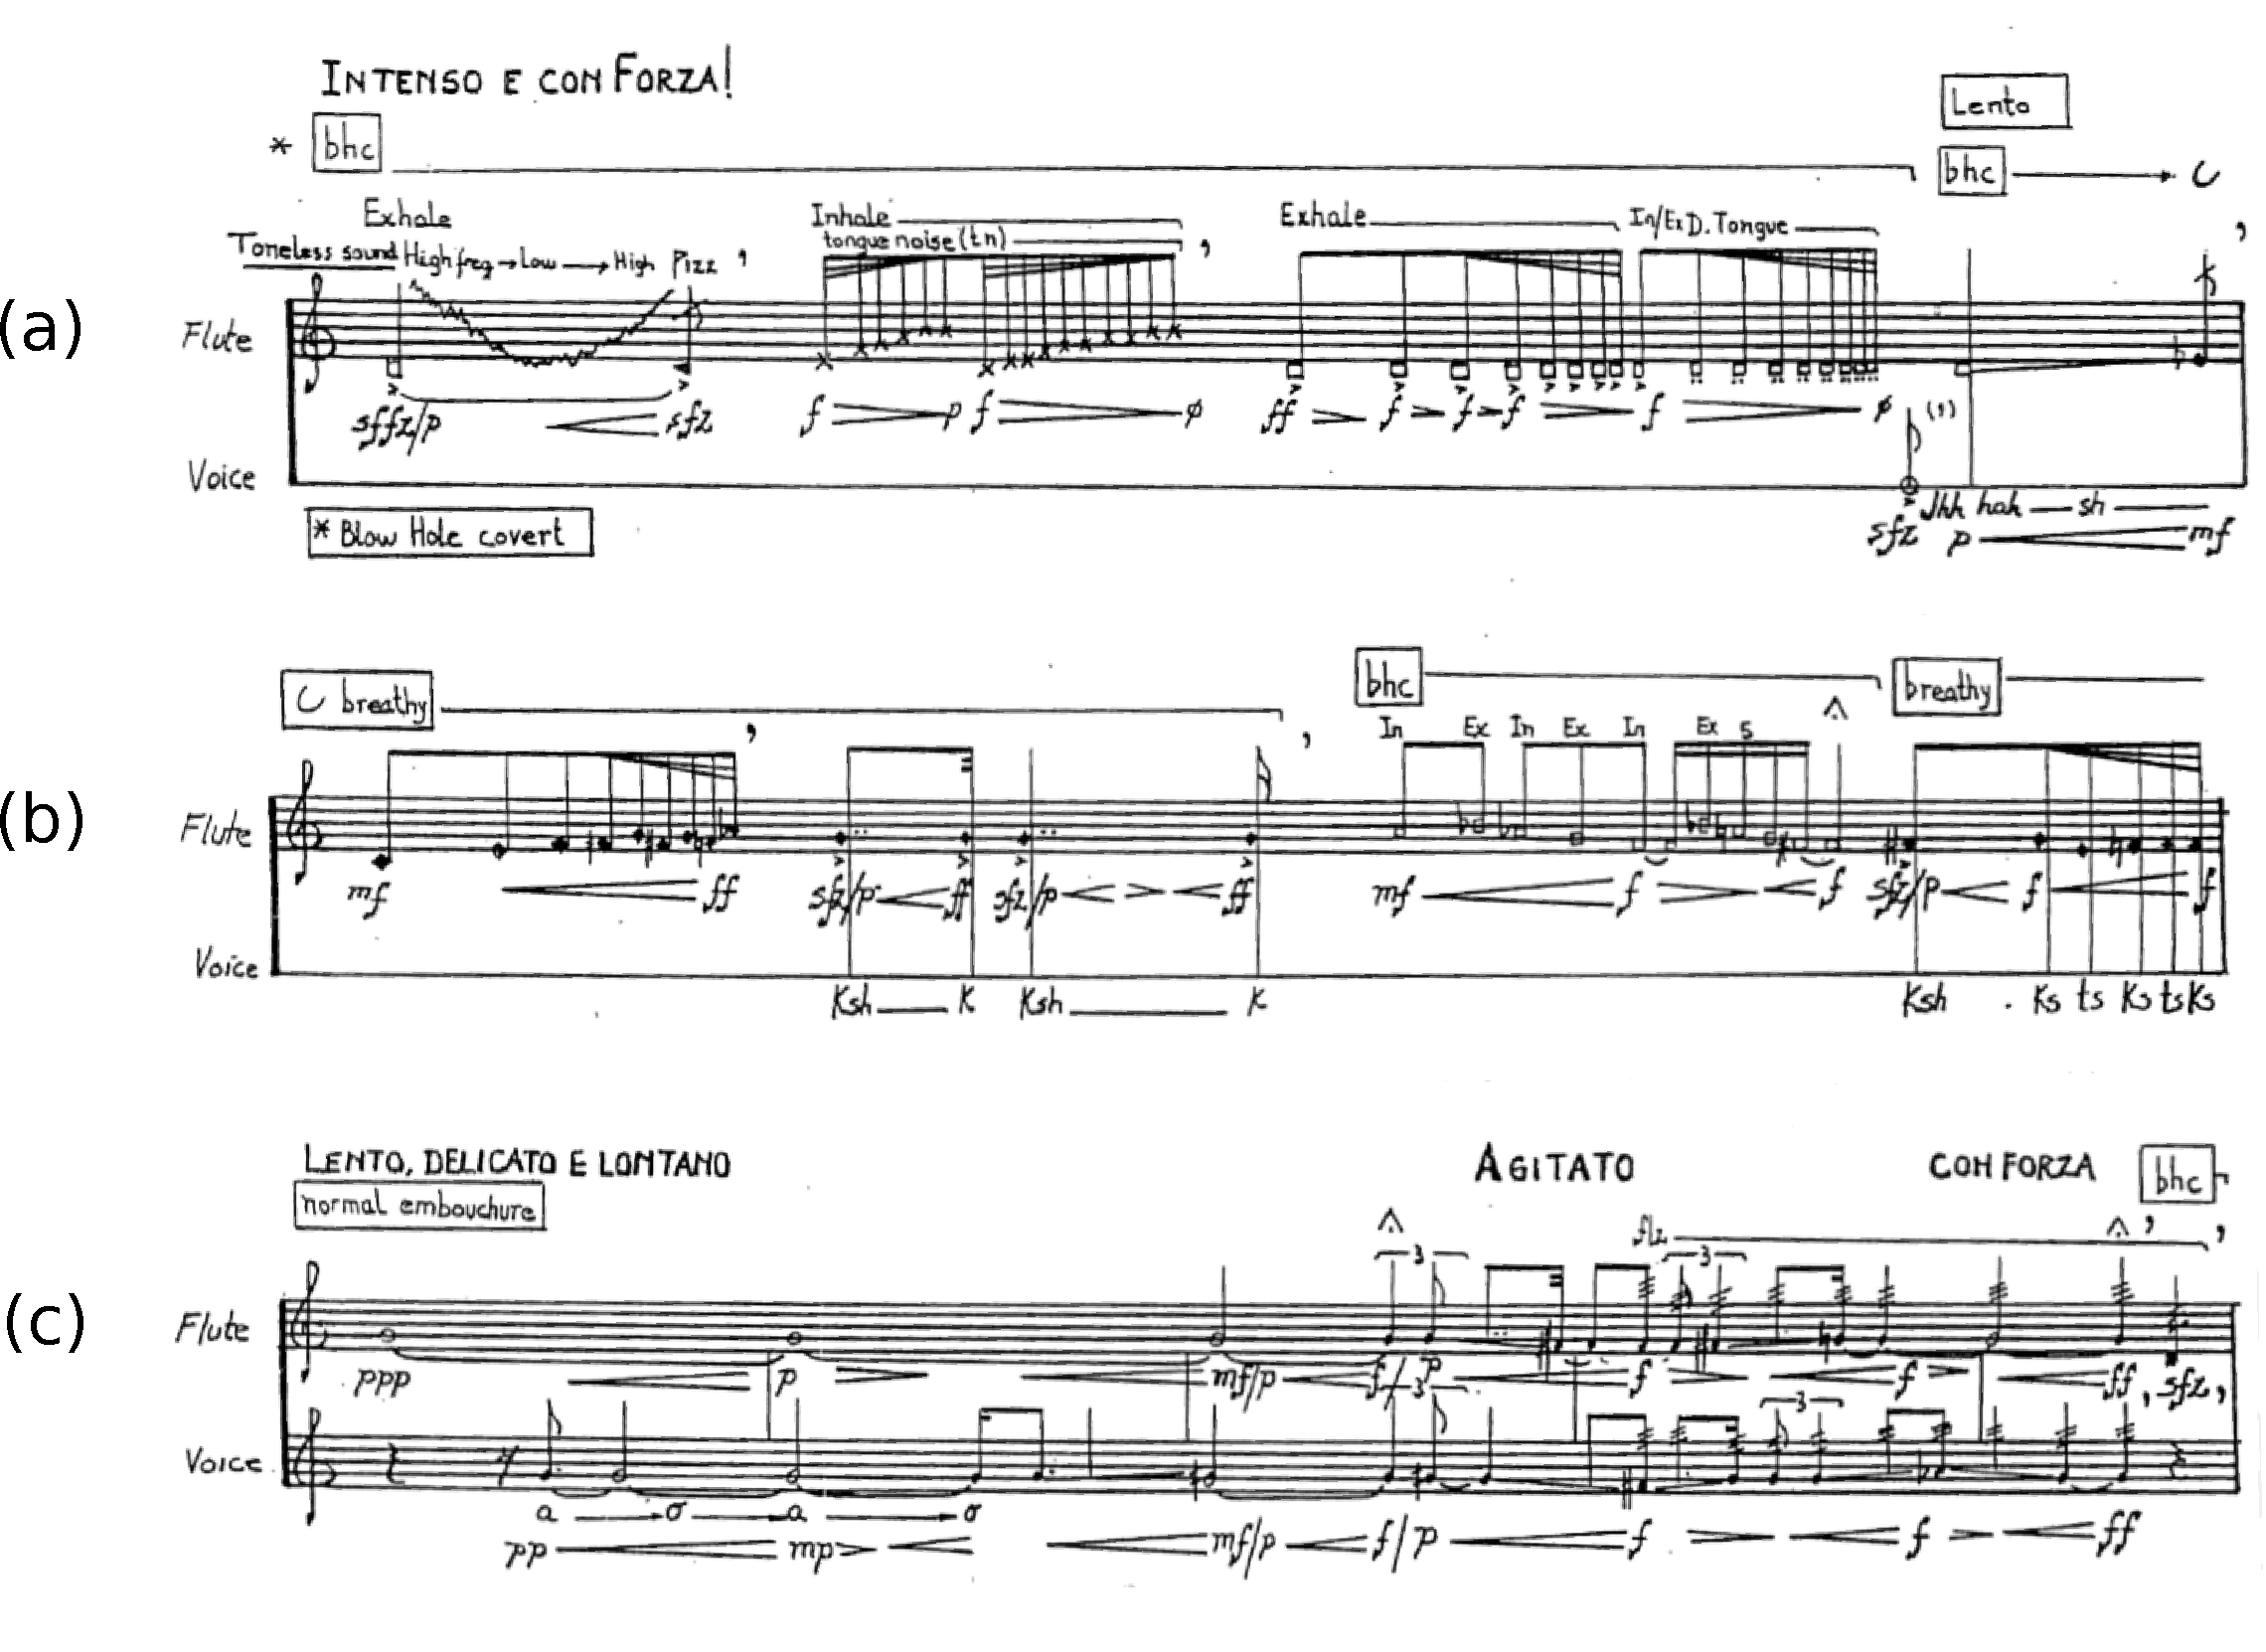
\includegraphics[width=0.9\textwidth]{embocaduras} 
\caption{Notación de las embocaduras se observa en la parte superior de los sistemas. (a) \textit{Blow Hole Covered}. (b) \textit{Breathy Embrochure}. (c) \textit{Normal Embrochure}. Fragmentos extraídos de la partitura de Aliento/Arrugas.}
\label{fig:embocaduras}
\end{center}
\end{figure}

\section*{Definición del Problema}
Se propone la extracción automática del tipo de embocadura a través del análisis computacional de grabaciones de la obra. En este caso se utilizará una estrategía de resolución del tipo de reconocimiento de patrones, en particular de clasificación supervisada. 

\section*{Datos}
Se cuenta con 3 grabaciones de diferentes intérpretes de la obra Aliento/Arrugas. Los intérpretes son: Pablo Somma, Emma Resmini y Ulla Suokko. Los archivos de audio se etiquetaron utilizando el software \textit{Sonic Visualizer} dividiendo los fragmentos de audio en 5 clases:

\begin{itemize} 
  \item Silencio.
  \item Silencio con respiración del intérprete. 
  \item Sonido generado con \textit{Blow Hole Covered}.
  \item Sonido generado con \textit{Breathy Embrochure}.
  \item Sonido generado con \textit{Normal Embrochure}.
\end{itemize}


 

\section*{Extracción de características}

Para esto se supone que el grado de tonalidad permite caracterizar el material sonoro generado con cada embocadura. Se enlista a continuación de forma cualitativa el grado de tonalidad con la respectiva embocadura:

\begin{itemize} 
  \item \textit{Blow Hole Covered}: Sonido atonal.
  \item \textit{Breathy Embrochure}: Sonido semi-tonal. 
  \item \textit{Normal Embrochure}: Sondio tonal.
\end{itemize}

Se propone entonces las utilización de dos características de audio clásicas para inferir el grado de tonalidad del material sonoro, desde las muestras digitales de audio: 

\begin{itemize} 
  \item \textit{Voicing} \cite[Chapter~12]{klapuri2007signal}.
  \item \textit{Zero-Crossing Rate} \cite[Chapter~4]{rabiner1978digital}. 
\end{itemize}
\medskip

Se supone entonces que mediante el computo de estas características es posible distinguir entre clases. A continuación se presentan los resultados y conclusiones sobre la estrategia planteada para la extracción de embocadura a partir del audio.

\newpage

\section*{Resultados}
Para el cálculo se utilizan ventanas de análisis de $23ms$ y saltos del $50\%$ del largo de la ventana. Se dejaron afuera del análisis las clases: \textit{Silencio} y \textit{Silencio con respiración del intérprete}.
\medskip

A continuación en la Figuras \ref{fig:histogramas_artista} y \ref{fig:comparative} se observa el espacio de características con distinción por clase para los diferentes intérpretes. Se puede observar que la \textit{Normal Embrochure} es separable frente al resto con estos cálculos. No es así el caso de las embocaduras \textit{Blow Hole Covered} y \textit{Breathy Embrocuhre}.

\begin{figure}[H]
\begin{center}
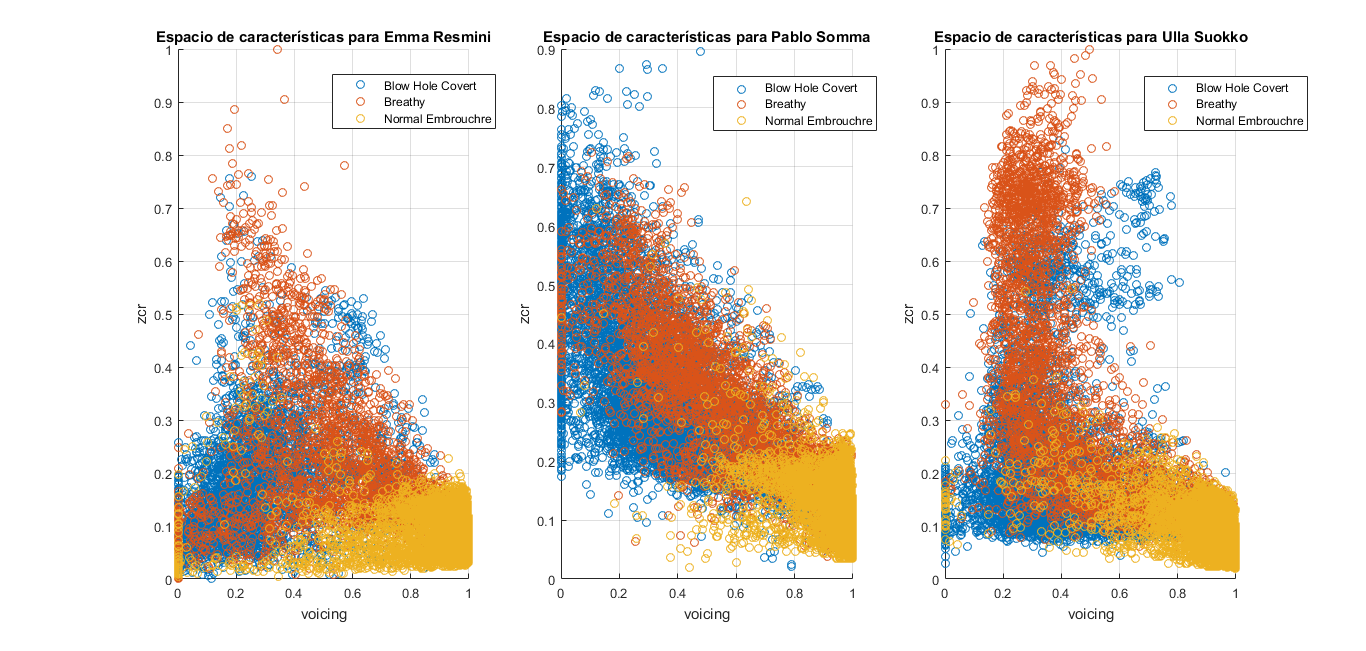
\includegraphics[width=1\textwidth]{histograms_artist} 
\caption{Espacio de características etiquetado por clases para cada uno de las interpretaciones.}
\label{fig:histogramas_artista}
\end{center}
\end{figure}

\begin{figure}[H]
\begin{center}
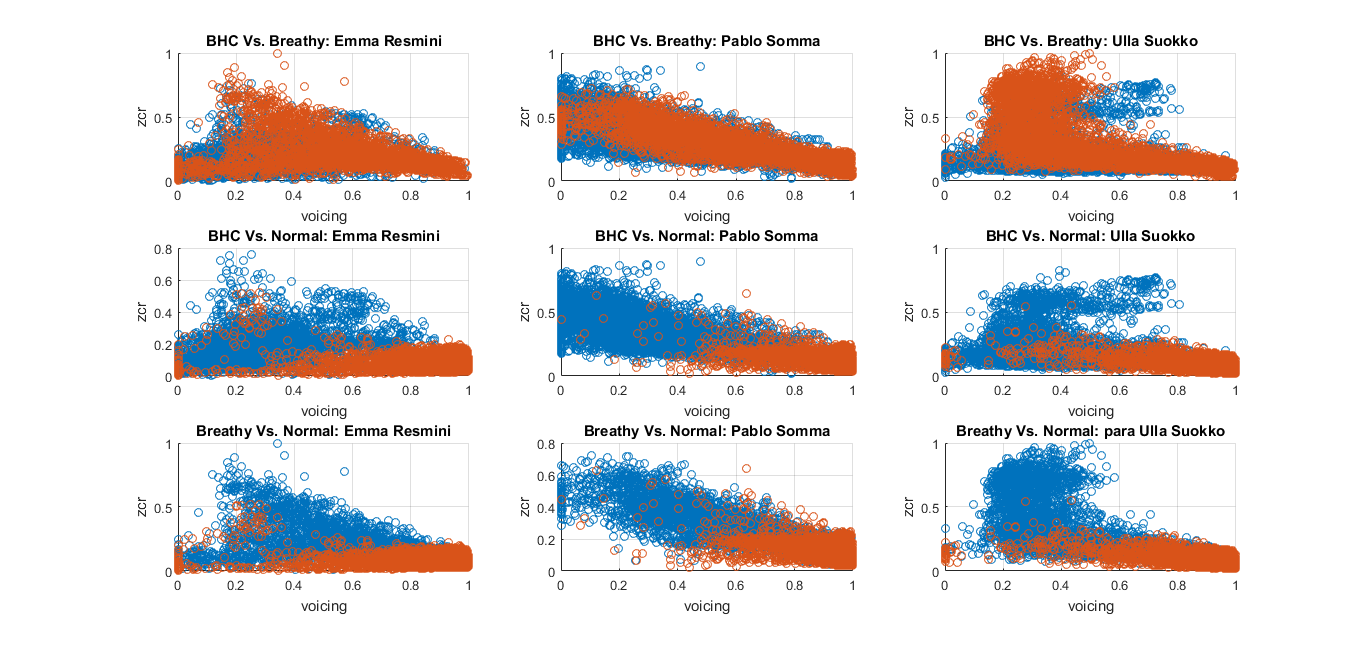
\includegraphics[width=1\textwidth]{comparative} 
\caption{Comparación clase vs. clase en el espacio de características.}
\label{fig:comparative}
\end{center}
\end{figure}

\newpage


Se observa además en las Figuras \ref{fig:bhc_features}, \ref{fig:breathyemb_features} y \ref{fig:normalemb_features} el comportamiento temporal de las características \textit{Voicing} y \textit{Zero-Crossing Rate} superpuestas con el espectrograma, para tres fragmentos de la interpretación de Emma Resmini. Corresponden a \textit{Blow Hole Covered}, \textit{Breathy Embrochure} y \textit{Normal Embrochure} respectivamente. Se corrobora lo dicho anteriormente sobre la separabilidad entre clases.

\begin{figure}[H]
\begin{center}
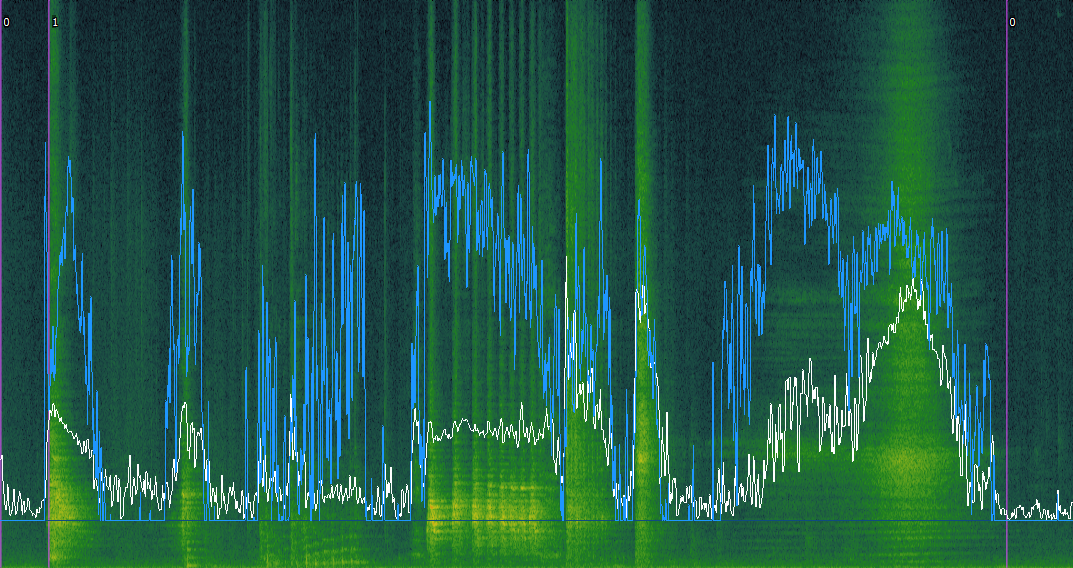
\includegraphics[width=1\textwidth]{bhc_features} 
\caption{Visualización de un fragmento de la interpretación de Emma Resmini con embocadura \textit{Blow Hole Covered}. Se observa en celeste el \textit{Voicing} y en blanco \textit{Zero-Crossing Rate}.}
\label{fig:bhc_features}
\end{center}
\end{figure}


\begin{figure}[H]
\begin{center}
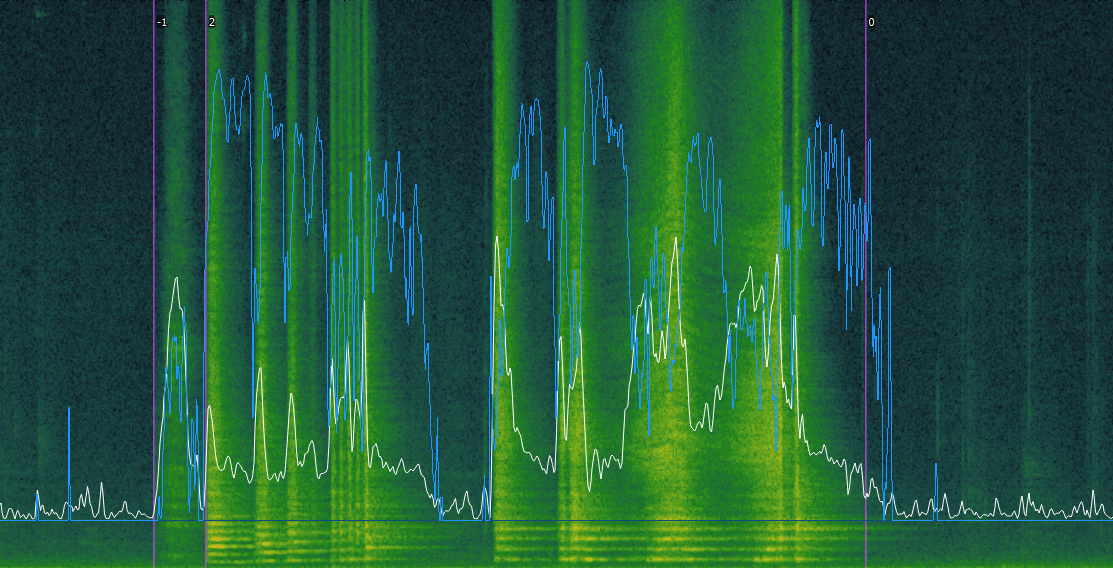
\includegraphics[width=1\textwidth]{breathyemb_features} 
\caption{Visualización de un fragmento de la interpretación de Emma Resmini con embocadura \textit{Breathy Embrochure}. Se observa en celeste el \textit{Voicing} y en blanco \textit{Zero-Crossing Rate}.}
\label{fig:breathyemb_features}
\end{center}
\end{figure}


\begin{figure}[H]
\begin{center}
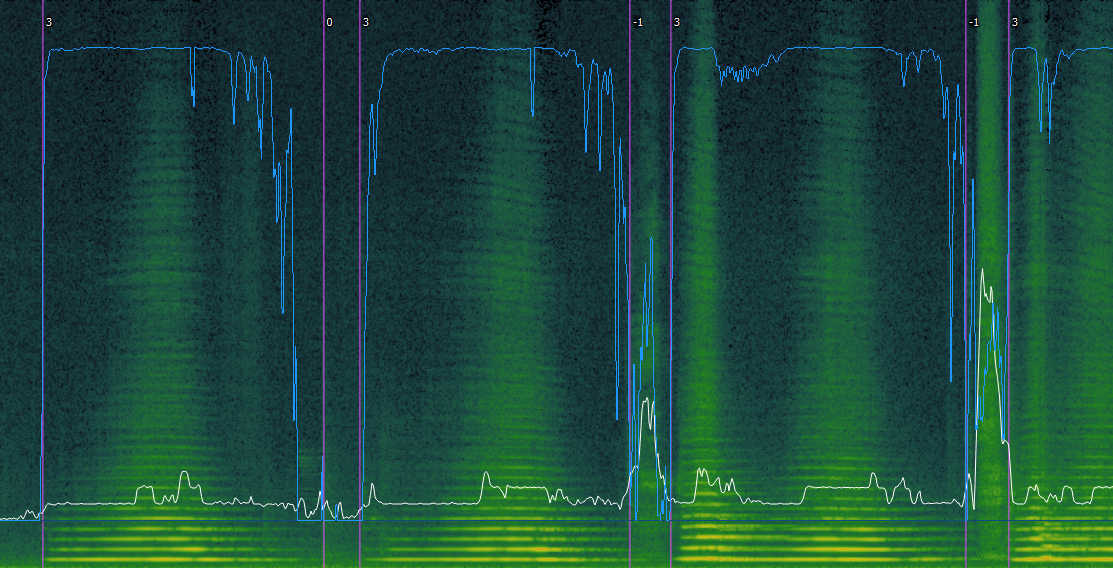
\includegraphics[width=1\textwidth]{normalemb_features} 
\caption{Visualización de un fragmento de la interpretación de Emma Resmini con embocadura \textit{Normal Embrochure}. Se observa en celeste el \textit{Voicing} y en blanco \textit{Zero-Crossing Rate}.}
\label{fig:normalemb_features}
\end{center}
\end{figure}

\section*{Conclusiones}

Las clases definidas por las embocaduras \textit{Breathy Embrochure} y \textit{Blow Hole Covered} no son separables en el espacio de características presentando en el informe. Por el contrario \textit{Normal Embrochure} se distingue del resto.  

%----------------------------------------------------------------------------------------
%	BIBLIOGRAPHY
%----------------------------------------------------------------------------------------


\newpage
\bibliographystyle{apalike}
\bibliography{biblio}


%----------------------------------------------------------------------------------------
\end{document}


